\documentclass[10pt]{beamer}

\usetheme{m}
\renewcommand{\mthemetitleformat}{\scshape\MakeLowercase}

\usepackage[ngerman]{babel}

\usepackage{booktabs}
\usepackage[scale=2]{ccicons}
\usepackage{alltt}
\usepackage{pifont}
\usepackage{marvosym}


\usepackage{tikz}
\usetikzlibrary{shapes,snakes}

\usepgfplotslibrary{dateplot}

\usepackage{xcolor}
\definecolor{dkgreen}{rgb}{0,0.6,0}
\definecolor{gray}{rgb}{0.5,0.5,0.5}
\definecolor{mauve}{rgb}{0.58,0,0.82}

\definecolor{gray}{rgb}{0.4,0.4,0.4}
\definecolor{darkblue}{rgb}{0.0,0.0,0.6}
\definecolor{cyan}{rgb}{0.0,0.6,0.6}


\setbeamertemplate{navigation symbols}{}
\setbeamertemplate{footline}
{
  \leavevmode%
  \hbox{%
  \begin{beamercolorbox}[wd=.333333\paperwidth,ht=2.25ex,dp=1ex,center]{author in head/foot}%
    \usebeamerfont{author in head/foot}\insertshortauthor%%%%~~(\insertshortinstitute)
  \end{beamercolorbox}%
  \begin{beamercolorbox}[wd=.333333\paperwidth,ht=2.25ex,dp=1ex,center]{author in head/foot}%
    \usebeamerfont{title in head/foot}\insertshorttitle
  \end{beamercolorbox}%
  \begin{beamercolorbox}[wd=.333333\paperwidth,ht=2.25ex,dp=1ex,right]{author in head/foot}%
    \usebeamerfont{date in head/foot}\insertshortdate{}\hspace*{6em}
    %\insertframenumber{} / \inserttotalframenumber\hspace*{2ex} 
    \insertframenumber{}\hspace*{12ex} 
  \end{beamercolorbox}}%
  \vskip0pt%
}

\title{Betriebliche Informationssysteme}
\subtitle{Präsentation der Ergebnisse im Praktikum \\[0.8cm] \LARGE{Angriffe auf AMQP-Messagebroker} \tiny{PT03}}
\date{6. Juli 2015}
\author{Philipp Sieder, Marcel Mielke}
\institute{Hochschule für Technik, Wirtschaft und Kultur Leipzig / Universität Leipzig}

\newcommand{\ok}{\textcolor{green}{\ding{52}}}
\newcommand{\nok}{\textcolor{red}{\ding{54}}}

\begin{document}

\maketitle

%############################################################

\section{Aufgabenstellung}

\subsection{}
\begin{frame}{Überblick}

	\begin{itemize}
		\item AMQP als Kommunikationsprotokoll für Message-orientierte Middleware (MOM)
		\item Demonstration von Angriffen auf Verfügbarkeit von AMQP-Brokern
		\begin{itemize}
			\item Auf Basis der Open Source Message Broker Software \glqq RabbitMQ\grqq
			\item Geschrieben in der Programmiersprache Erlang
		\end{itemize}
		\item Fokus auf Denial-of-Service
	\end{itemize}
	
	\begin{center}
		
\includegraphics[width=0.3\textwidth]{pic/rabbit_logo}
	\end{center}
		
\end{frame}

%----------------------------------------------------------------------

\begin{frame}{Beispiel}
	\begin{center}
		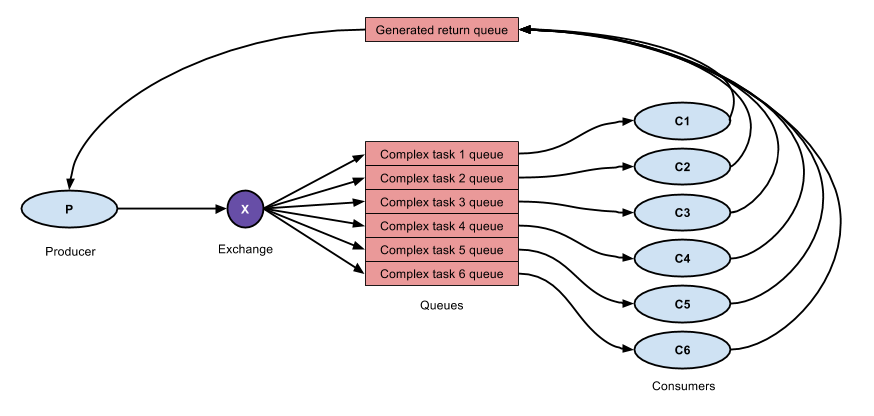
\includegraphics[width=\textwidth]{pic/over}
	\end{center}
\end{frame}

\subsection{}
\begin{frame}{Rahmenbedingungen}
	\begin{itemize}
		\item Identifikation und Bewertung potenzieller Angriffsvektoren auf AMQP, RabbitMQ
		\item Messung von Latenz, Speicher, CPU-Auslastung, ...
		\item Implementierung von Beispielen auf Basis der RabbitMQ Java Client Library
		\item Vorschläge für Schadensbegrenzung
	\end{itemize}
\end{frame}

%----------------------------------------------------------------------

\begin{frame}{Identifikation von Angriffsvektoren}
	\begin{itemize}
		\item Viele Verbindungen
		\item Bruteforce-Attacke auf Benutzercredentials
		\item Hohe Datenrate (viele kleine, wenig große Nachrichten)
		\item Große Header, kleiner Payload
		\item Langsamer Verbindungsaufbau
		\item Unvollständiger Verbindungsaufbau
		\item Pause im Protokollablauf
	\end{itemize}
\end{frame}



%################################################################%
% ####################### Werkzeuge ############################ %
%################################################################%
\section{Werkzeuge}


\begin{frame}{VirtualBox}
	\begin{itemize}
		\item Konfiguration der virtuellen Hardware
		\item Erstellung von Sicherungspunkten 
		\item Portabilität der Testumgebung
		\item Als Grundlage dient die Servervariante von Ubuntu 14.04.2 LTS
	\end{itemize}
	\begin{figure}
		\vspace{-0.5cm}
		\centering
		
\includegraphics[width=\textwidth]{pic/virtual-box}
	\end{figure}	
\end{frame}

%------------------------------------------------

\begin{frame}{Glances}
	\begin{figure}
		\vspace{-0.5cm}
		\centering
		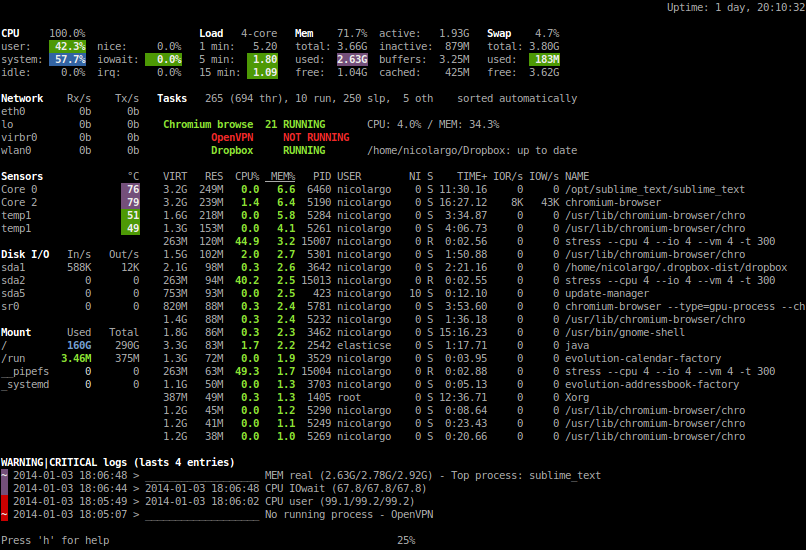
\includegraphics[width=\textwidth]{pic/glances}
	\end{figure}
\end{frame}

%------------------------------------------------

\begin{frame}{RabbitMQ Management Tool (I)}
	\begin{figure}
		\vspace{-0.5cm}
		\centering
		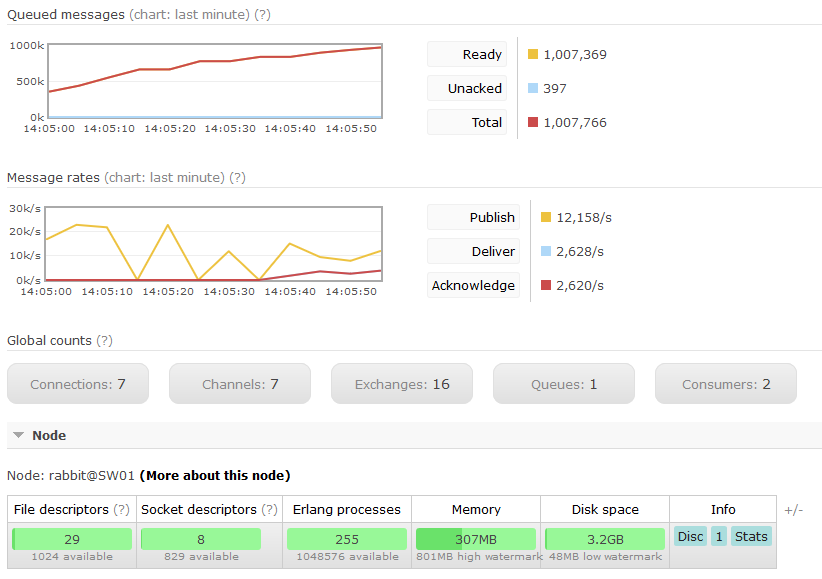
\includegraphics[width=\textwidth]{pic/rmqoverview}
	\end{figure}
\end{frame}

\begin{frame}{RabbitMQ Management Tool (II)}
	\begin{figure}
		\vspace{-0.7cm}
		\centering
		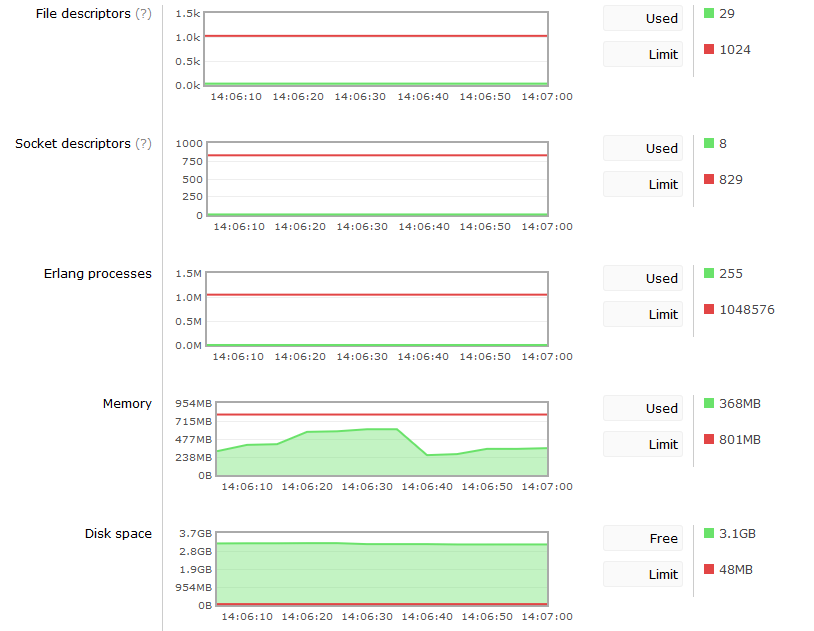
\includegraphics[width=0.95\textwidth]{pic/rmqoverview2}
	\end{figure}
\end{frame}

%------------------------------------------------

\begin{frame}{HTML Performance Tools}
	\begin{itemize}
		\item Definition von Anwendungsszenarien
		\item Verwendung von \textbf{PerfTest} (Bestandteil der RabbitMQ-Client-Bibliothek)
		\item automatisierte Ausführung
		\item Alle Ergebnisse werden in einer JSON-Datei gesichert und über HTML, JS, CSS visualisiert
		\item \url{https://github.com/rabbitmq/rabbitmq-perf-html}
	\end{itemize}
\end{frame}


%------------------------------------------------

\begin{frame}{AMQPstress}
	\centering
	\begin{itemize}
		\item Implementierung von Clients für mögliche Angriffsvektor
		\item Zahlreiche Einstellungsmöglichkeiten
		\item Projekt und Dokumentation zugänglich über GitHub
	\end{itemize}
  
	\begin{figure}[!htb]
	\centering
 		\fcolorbox{black}{gray}{
\includegraphics[width=0.33\textwidth]{pic/qrcode}}
		\\[0.2cm] https://github.com/philippsied/amqp-stress-test
	\label{fig1}
	\end{figure}
\end{frame}

\begin{frame}[t]{AMQPstress - Argumente}
	\begin{alltt}
		\tiny
		\input{other/pout.txt}
	\end{alltt}
\end{frame}

\subsection{}
%------------------------------------------------

\begin{frame}{Reporting}
	\centering
	\begin{itemize}
		\item Aggregation der Informationen und Visualisierung aller Messergebnisse
		\item Verwendet Web-Technologien
		\item basiert auf der Visualisierung der HTML Performance Tools
	\end{itemize}
  
	\begin{figure}[!htb]
		\centering
 		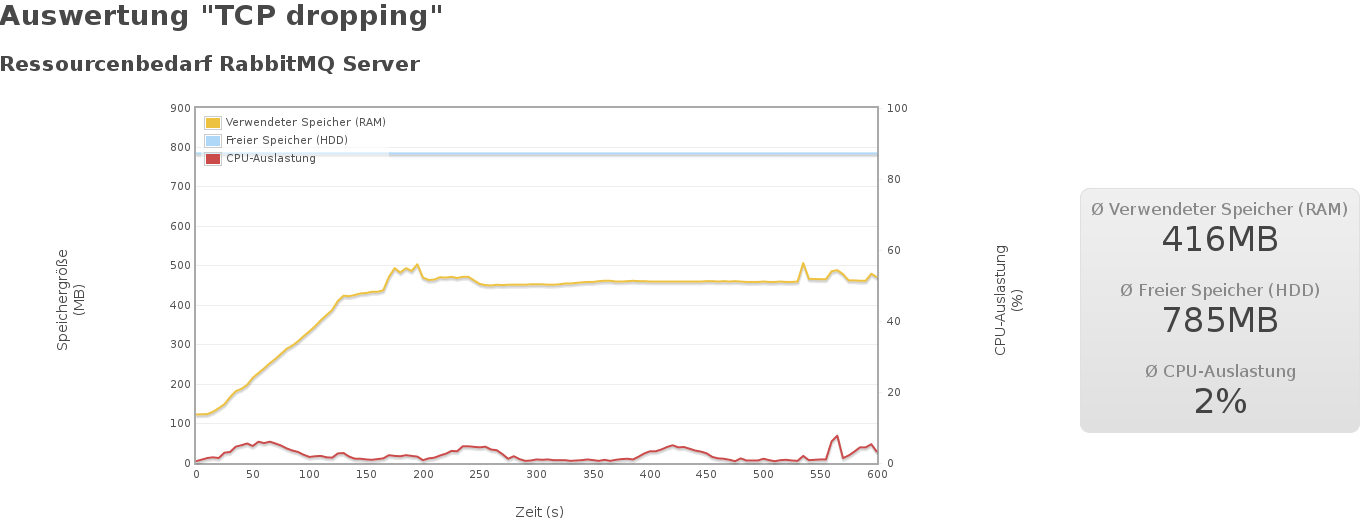
\includegraphics[width=\textwidth]{pic/reporting.png}
	\end{figure}
\end{frame}




%################################################################%
% ####################### Angriffe ############################# %
%################################################################%
\section{Angriffe}

%-------------------------------------------------------%
% ------------------ Channel-Flooding ----------------- %
%-------------------------------------------------------%
\begin{frame}[t]{Angriff - Channel-Flooding}
\begin{description}
	\item[Aktion:]
		\begin{enumerate}
			\item Client öffnet viele Channel auf \textsl{einer} Verbindung
			\item Client sendet Nachrichten über Channel
		\end{enumerate} \smallskip
	\item[Ziel:] CPU, RAM, Netzwerkbandbreite, Festplatte \smallskip
	\item[Ansatz:] Server muss für jeden Channel Ressourcen allokieren und die Kommunikation aufrechterhalten. Die Channel teilen sich dabei eine TCP-Verbindung.
\end{description}
\end{frame}

\begin{frame}{Angriff - Channel-Flooding}
\begin{figure}[!htb]
	\centering
	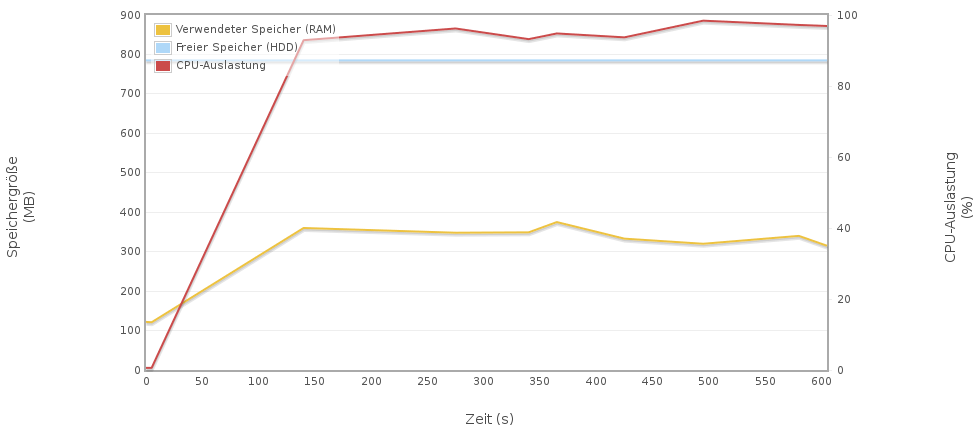
\includegraphics[width=\textwidth]{img/channel/channel_server1.png}
	\caption{\centering Channel-Flooding - Verlauf des Speicherbedarfs für RAM/HDD und Verlauf der CPU-Last auf dem RabbitMQ-Server}
	\label{fig:channel-server1}
\end{figure}
\end{frame}
	
\begin{frame}{Angriff - Channel-Flooding}
\begin{figure}[!htb]
	\centering
	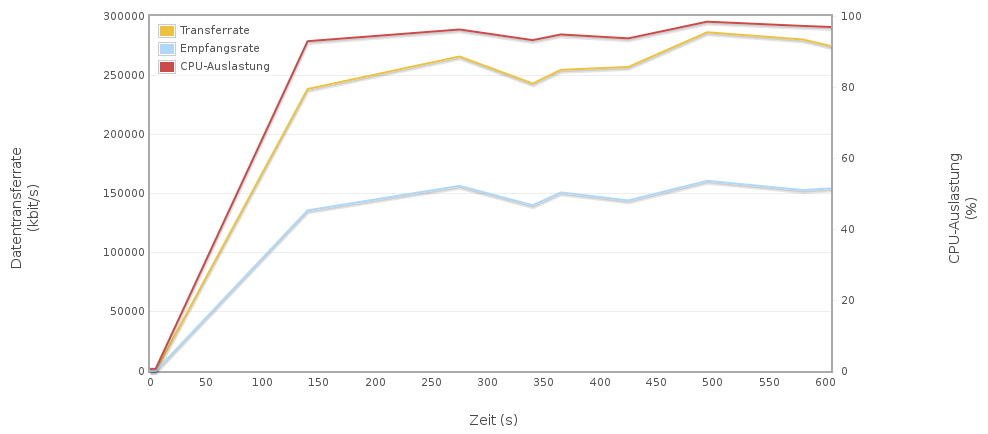
\includegraphics[width=\textwidth]{img/channel/channel_server2.png}
	\caption{\centering Channel-Flooding - Verlauf der Transfer-, Empfangsrate und Verlauf der CPU-Last auf dem RabbitMQ-Server}
	\label{fig:channel-server2}
\end{figure}
\end{frame}

\begin{frame}{Angriff - Channel-Flooding}	
\begin{figure}[!htb]
	\centering
	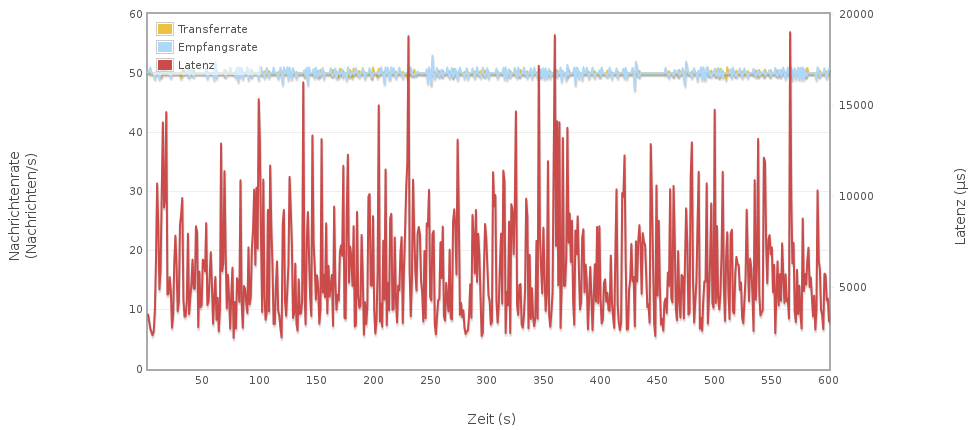
\includegraphics[width=\textwidth]{img/channel/channel_scenario.png}
	\caption{\centering Channel-Flooding - Verlauf der Transfer-, Empfangsrate und Verlauf der Latenz im Anwendungsszenario}
	\label{fig:channel-scenario}
\end{figure}
\end{frame}

\begin{frame}{Angriff - Channel-Flooding}
\begin{table}[!htb]
	\centering
	\begin{tabular}{p{3cm}llp{3cm}}
		Übertragungsrate\newline (schreiben) & Producer & Consumer & Nachrichtengröße\newline (Byte) \\ \hline
		7.000m/s                             & 100      & 10       & 100                              \\
		800m/s                               & 100      & 10       & 1.000                            \\
		100m/s                               & 100      & 10       & 10.000
	\end{tabular}
	\caption{Mehrere Channel}
\end{table}
\end{frame}

\begin{frame}{Angriff - Channel-Flooding}
\begin{table}[!htb]
	\centering
	\begin{tabular}{p{3cm}llp{3cm}}
		Übertragungsrate\newline (schreiben) & Producer & Consumer & Nachrichtengröße\newline (Byte) \\ \hline
		24.000m/s                            & 100      & 10       & 100                             \\
		2.000m/s                             & 100      & 10       & 1.000                           \\
		100m/s                               & 100      & 10       & 10.000
	\end{tabular}
	\caption{Mehrere Connections}
\end{table}
\end{frame}


%-------------------------------------------------------%
% ------------ Nachrichten mit großem Header ---------- %
%-------------------------------------------------------%
\begin{frame}[t]{Angriff - Versenden von Nachrichten mit großem Header}
\begin{description}
	\item[Aktion:]
		\begin{enumerate}
			\item Client erzeugt Nachrichten mit sehr großem Header
			\item Header enthält Weiterleitungsoption zu ungültigem Ziel
			\item Client sendet Nachricht an Server
		\end{enumerate} \smallskip
	\item[Ziel:] CPU, RAM, Festplatte \smallskip
	\item[Ansatz:] Server muss alle Headerinformationen prüfen, auch ungültige Ziele von Weiterleitungsoptionen. 
\end{description}
\end{frame}

\begin{frame}{Angriff - Versenden von Nachrichten mit großem Header}
\begin{figure}[!htb]
	\centering
	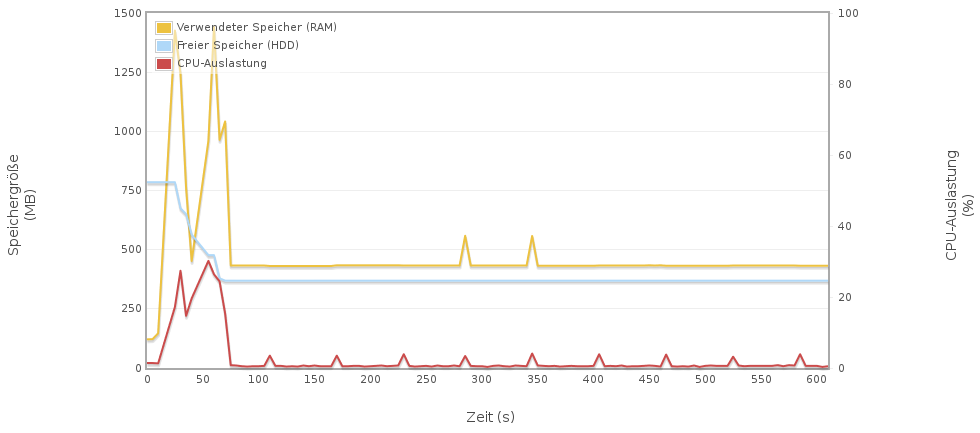
\includegraphics[width=\textwidth]{img/header/header_server1.png}
	\caption{\centering Nachrichten mit großem Header - Verlauf des Speicherbedarfs für RAM/HDD und Verlauf der CPU-Last auf dem RabbitMQ-Server}
	\label{fig:header-server1}
\end{figure}
\end{frame}
	
\begin{frame}{Angriff - Versenden von Nachrichten mit großem Header}	
\begin{figure}[!htb]
	\centering
	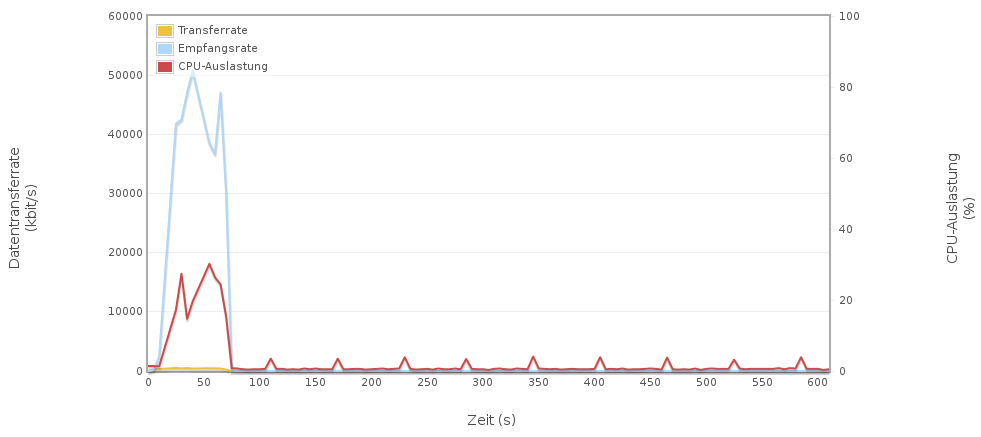
\includegraphics[width=\textwidth]{img/header/header_server2.png}
	\caption{\centering Nachrichten mit großem Header - Verlauf der Transfer-, Empfangsrate und Verlauf der CPU-Last auf dem RabbitMQ-Server}
	\label{fig:header-server2}
\end{figure}
\end{frame}

\begin{frame}{Angriff - Versenden von Nachrichten mit großem Header}	
\begin{block}{Keine Messung möglich}
Anwendung zum Testen des Szenarios konnte nicht beendet werden - Keine Messergebnisse
\end{block}
\end{frame}

\begin{frame}{Angriff - Versenden von Nachrichten mit großem Header}
\begin{table}[h]
	\centering
	\begin{tabular}{p{3cm}ll|p{3cm}}
		\multicolumn{3}{l|}{Übertragungsrate nach Nachrichtengröße}  & Headergröße     \\
		10.000 Byte          & 1.000 Byte              & 100 Byte    & Einträge (Byte) \\ \hline
		140m/s               & 260m/s                  & 350m/s      & 200 (8.800)     \\
		80m/s                & 120m/s                  & 180m/s      & 500 (22.000)    \\
		30m/s                & 50m/s                   & 70m/s       & 1.000 (44.000)  \\
		20m/s                & 30m/s                   & 40m/s       & 2.000 (88.000)  \\
		10m/s                & 10m/s                   & 20m/s       & 2.500 (110.000) \\ \hline
		270m/s              & 3000m/s              & 10000m/s & Kein Header \\
	\end{tabular}
\end{table}
\end{frame}

%-------------------------------------------------------%
% ------------------ Transaktionsmodus ---------------- %
%-------------------------------------------------------%
\begin{frame}[t]{Angriff - Transaktionsmodus}
\begin{description}
	\item[Aktion:]
		\begin{enumerate}
			\item Clients starten Transaktionen
			\item Clients senden Nachrichten an Server
			\item \textbf{Keiner} der Clients führt einen \textsl{commit} aus
		\end{enumerate} \smallskip
	\item[Ziel:] CPU, RAM \smallskip
	\item[Ansatz:] Server muss die Daten von Transaktionen zwischenspeichern bis ein \textsl{commit} oder ein \textsl{rollback} stattgefunden hat.
\end{description}
\end{frame}

\begin{frame}{Angriff - Transaktionsmodus}
\begin{figure}[!htb]
	\centering
	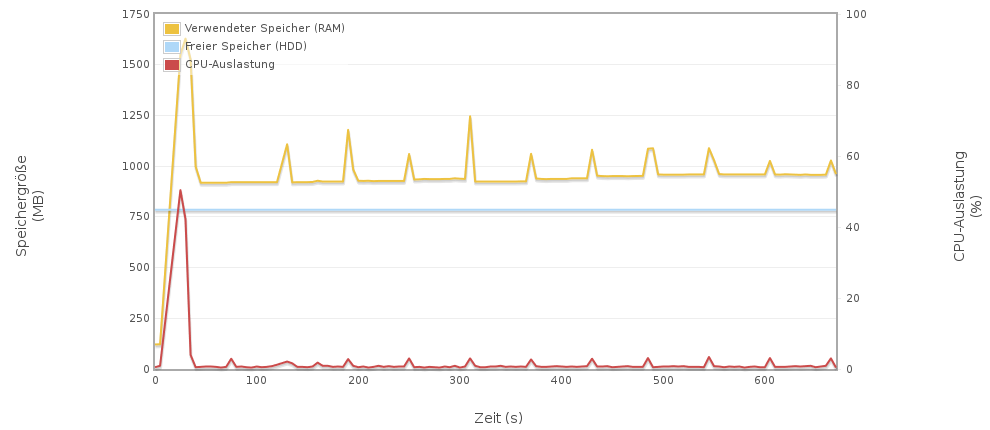
\includegraphics[width=\textwidth]{img/tx/tx_server1.png}
	\caption{\centering Ausbleiben von Commits im Transaktionsmodus - Verlauf des Speicherbedarfs für RAM/HDD und Verlauf der CPU-Last auf dem RabbitMQ-Server}
	\label{fig:tx-server1}
\end{figure}
\end{frame}

\begin{frame}{Angriff - Transaktionsmodus}		
\begin{figure}[!htb]
	\centering
	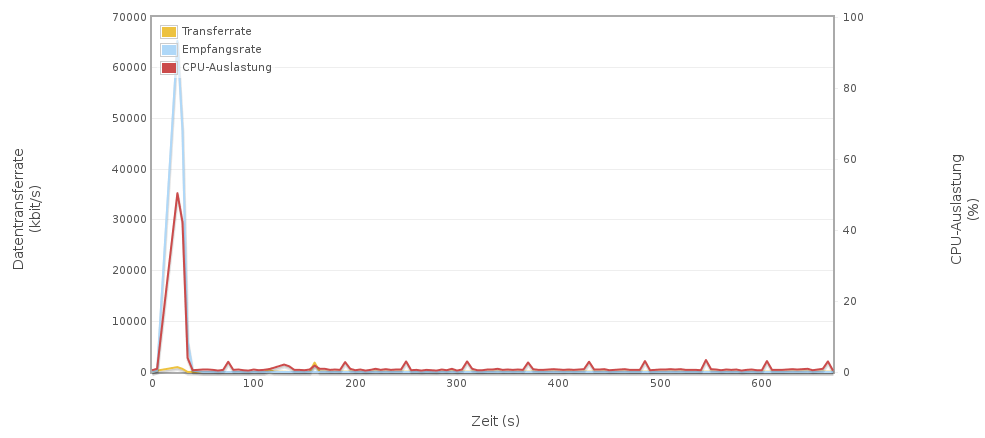
\includegraphics[width=\textwidth]{img/tx/tx_server2.png}
	\caption{\centering Ausbleiben von Commits im Transaktionsmodus - Verlauf der Transfer-, Empfangsrate und Verlauf der CPU-Last auf dem RabbitMQ-Server}
	\label{fig:tx-server2}
\end{figure}
\end{frame}

\begin{frame}{Angriff - Transaktionsmodus}	
\begin{block}{Keine Messung möglich}
Anwendung zum Testen des Szenarios konnte nicht beendet werden - Keine Messergebnisse
\end{block}
\end{frame}

%-------------------------------------------------------%
% ------------- Ignorieren von Nachrichten ------------ %
%-------------------------------------------------------%
\begin{frame}[t]{Angriff - Ignorieren von Nachrichten}
\begin{description}
	\item[Aktion:]
		\begin{enumerate}
			\item Producer sendet Nachrichten an Server
			\item Mehrere Consumer erhalten Nachrichten
			\item Consumer ignorieren die Quittierung
		\end{enumerate} \smallskip
	\item[Ziel:] RAM, Festplatte
	\item[Ansatz:] Server muss alle Nachrichten zwischenspeichern bis der Erhalt quittiert wurde.
\end{description}
\end{frame}

\begin{frame}{Angriff - Ignorieren von Nachrichten}
\begin{figure}[!htb]
	\centering
	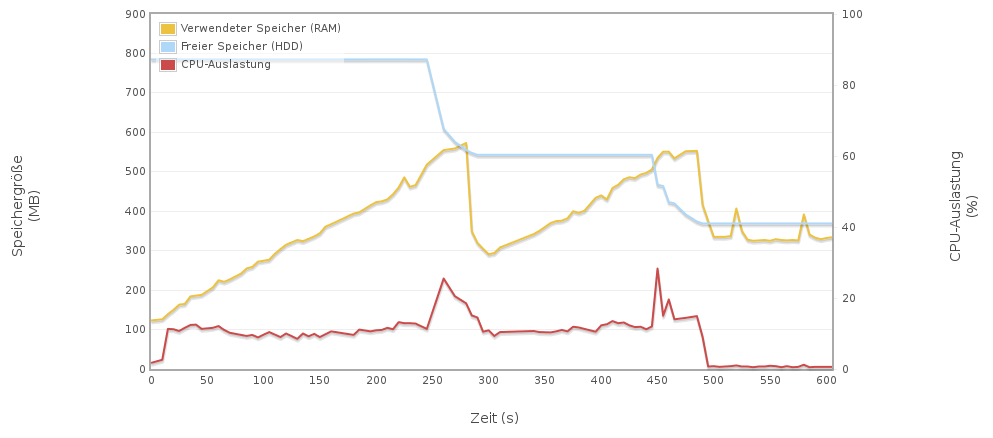
\includegraphics[width=\textwidth]{img/no/no_server1.png}
	\caption{\centering Ignorieren von Nachrichten - Verlauf des Speicherbedarfs für RAM/HDD und Verlauf der CPU-Last auf dem RabbitMQ-Server}
	\label{fig:no-server1}
\end{figure}	
\end{frame}

\begin{frame}{Angriff - Ignorieren von Nachrichten}	
\begin{figure}[!htb]
	\centering
	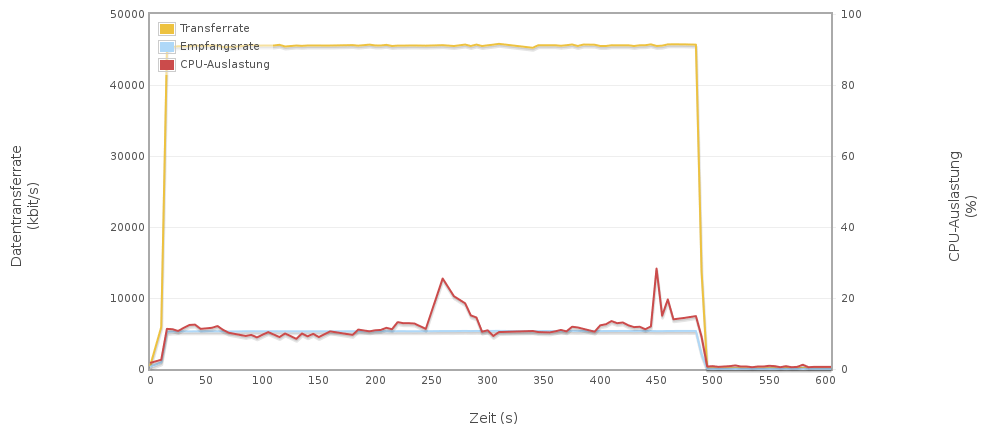
\includegraphics[width=\textwidth]{img/no/no_server2.png}
	\caption{\centering Ignorieren von Nachrichten - Verlauf der Transfer-, Empfangsrate und Verlauf der CPU-Last auf dem RabbitMQ-Server}
	\label{fig:no-server2}
\end{figure}		
\end{frame}

\begin{frame}{Angriff - Ignorieren von Nachrichten}	
\begin{figure}[!htb]
	\centering
	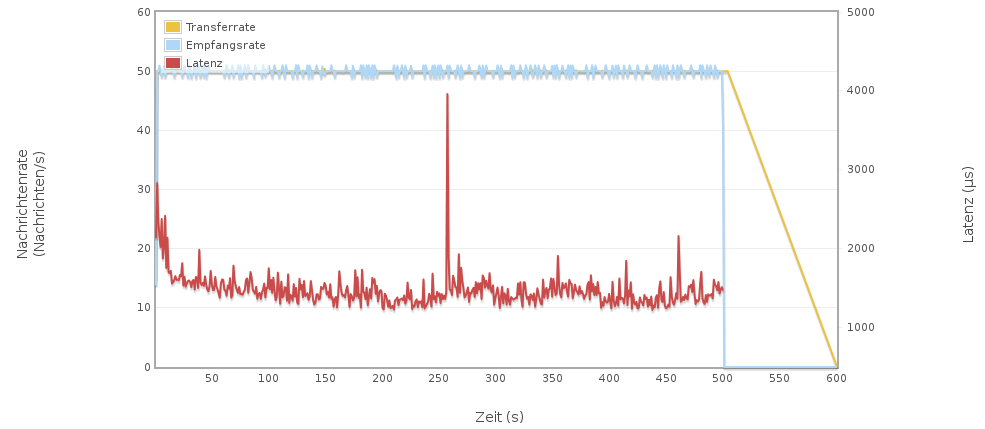
\includegraphics[width=\textwidth]{img/no/no_scenario.png}
	\caption{\centering Ignorieren von Nachrichten - Verlauf der Transfer-, Empfangsrate und Verlauf der Latenz im Anwendungsszenario}
	\label{fig:no-scenario}
\end{figure}
\end{frame}


%-------------------------------------------------------%
% -------- Sofortiges Abweisen von Nachrichten -------- %
%-------------------------------------------------------%
\begin{frame}[t]{Angriff - Sofortiges Abweisen von Nachrichten}
\begin{description}
	\item[Aktion:]
		\begin{enumerate}
			\item Producer sendet Nachrichten an Server
			\item Mehrere Consumer erhalten Nachrichten
			\item Consumer senden jedoch sofort eine \textsl{Negative Bestätigung}
		\end{enumerate} \smallskip
	\item[Ziel:] RAM, Festplatte, Netzwerkbandbreite \smallskip
	\item[Ansatz:] Server muss alle Nachrichten zwischenspeichern bis der Erhalt \textsl{erfolgreich} quittiert wurde und muss abgewiesene Nachrichten erneut senden.
\end{description}
\end{frame}

\begin{frame}{Angriff - Sofortiges Abweisen von Nachrichten}
\begin{figure}[!htb]
	\centering
	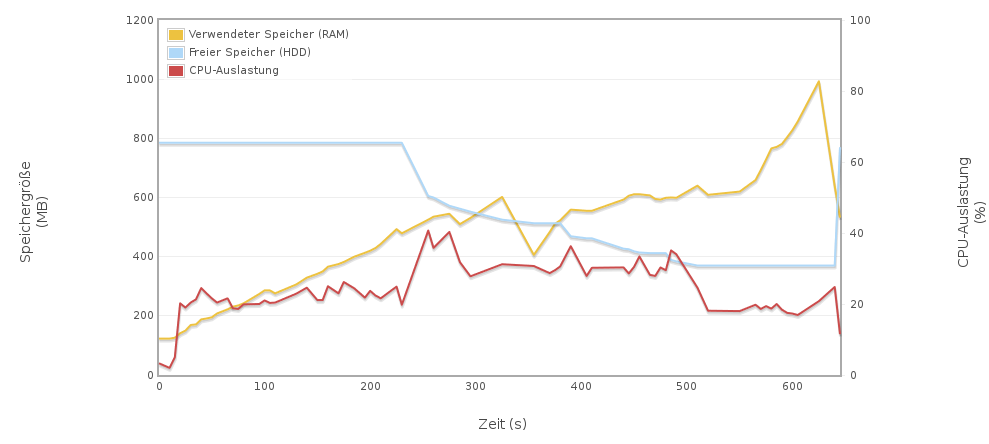
\includegraphics[width=\textwidth]{img/reject/reject_server1.png}
	\caption{\centering Sofortiges Abweisen von Nachrichten - Verlauf des Speicherbedarfs für RAM/HDD und Verlauf der CPU-Last auf dem RabbitMQ-Server}
	\label{fig:reject-server1}
\end{figure}
\end{frame}

\begin{frame}{Angriff - Sofortiges Abweisen von Nachrichten}		
\begin{figure}[!htb]
	\centering
	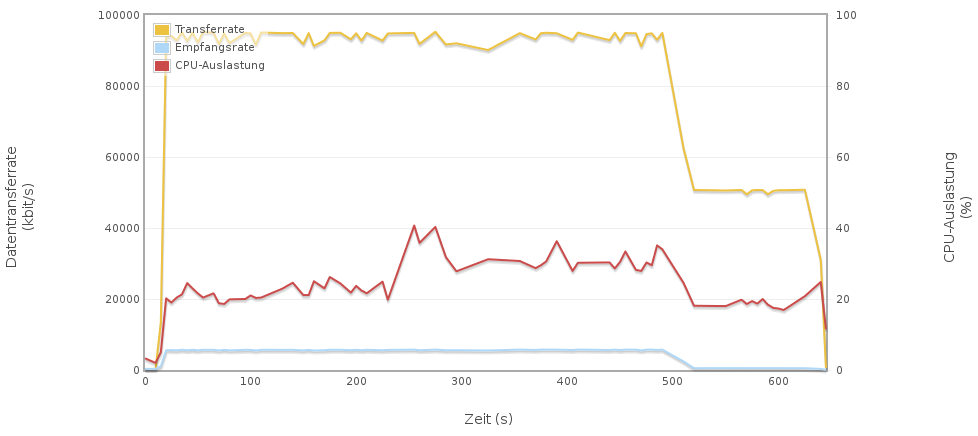
\includegraphics[width=\textwidth]{img/reject/reject_server2.png}
	\caption{\centering Sofortiges Abweisen von Nachrichten - Verlauf der Transfer-, Empfangsrate und Verlauf der CPU-Last auf dem RabbitMQ-Server}
	\label{fig:reject-server2}
\end{figure}
\end{frame}

\begin{frame}{Angriff - Sofortiges Abweisen von Nachrichten}		
\begin{figure}[!htb]
	\centering
	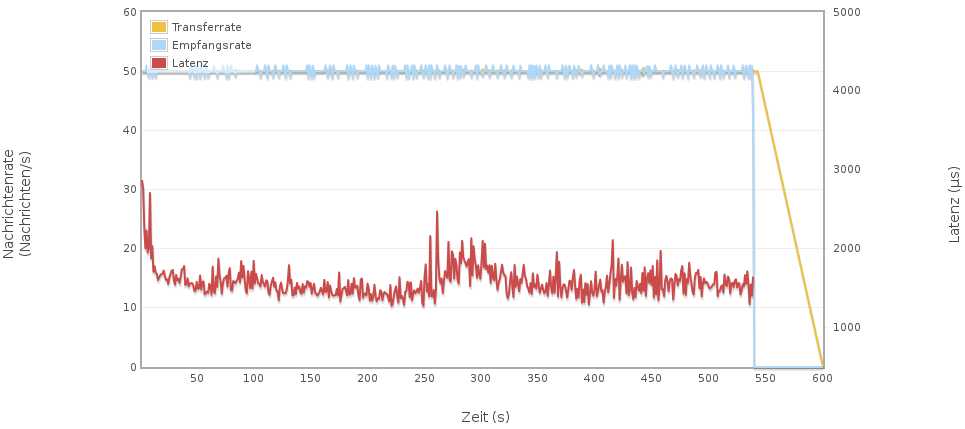
\includegraphics[width=\textwidth]{img/reject/reject_scenario.png}
	\caption{\centering Sofortiges Abweisen von Nachrichten - Verlauf der Transfer-, Empfangsrate und Verlauf der Latenz im Anwendungsszenario}
	\label{fig:reject-scenario}
\end{figure}
\end{frame}

%-------------------------------------------------------%
% ------- Gebündeltes Abweisen von Nachrichten -------- %
%-------------------------------------------------------%
\begin{frame}[t]{Angriff - Gebündeltes Abweisen von Nachrichten}
\begin{description}
	\item[Aktion:]
		\begin{enumerate}
			\item Producer sendet Nachrichten an Server
			\item Mehrere Consumer erhalten Nachrichten
			\item Consumer ignorieren diese bis um Erreichen eines Schwellwertes
			\item Alle empfangen Nachrichten werden \textsl{gebündelt} über eine \textsl{Negative Bestätigung} abgewiesen 
		\end{enumerate}  \smallskip
	\item[Ziel:] RAM, Festplatte, Netzwerkbandbreite, CPU \smallskip
	\item[Ansatz:] Server muss alle Nachrichten zwischenspeichern bis der Erhalt \textsl{erfolgreich} quittiert wurde und muss alle abgewiesene Nachrichten \textsl{stoßweise} erneut senden.
\end{description}
\end{frame}

\begin{frame}{Angriff - Gebündeltes Abweisen von Nachrichten}
\begin{figure}[!htb]
	\centering
	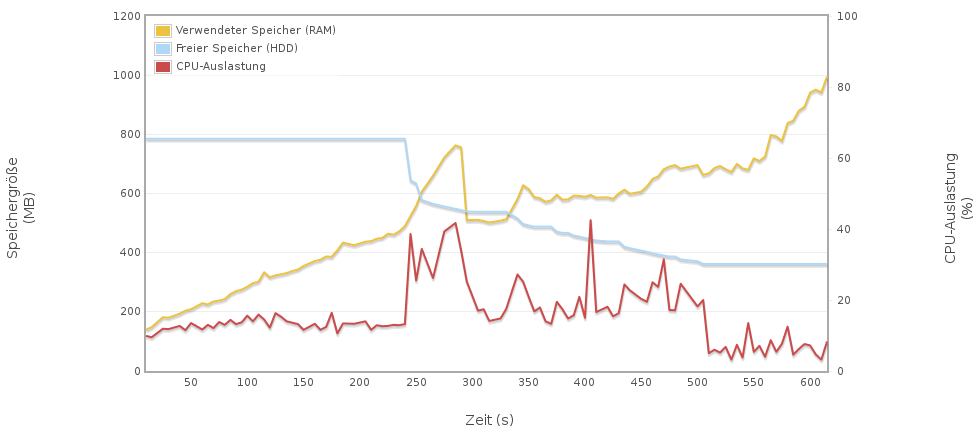
\includegraphics[width=\textwidth]{img/nack/nack_server1.png}
	\caption{\centering Gebündeltes Abweisen von Nachrichten - Verlauf des Speicherbedarfs für RAM/HDD und Verlauf der CPU-Last auf dem RabbitMQ-Server}
	\label{fig:nack-server1}
\end{figure}
\end{frame}
		
\begin{frame}{Angriff - Gebündeltes Abweisen von Nachrichten}
\begin{figure}[!htb]
	\centering
	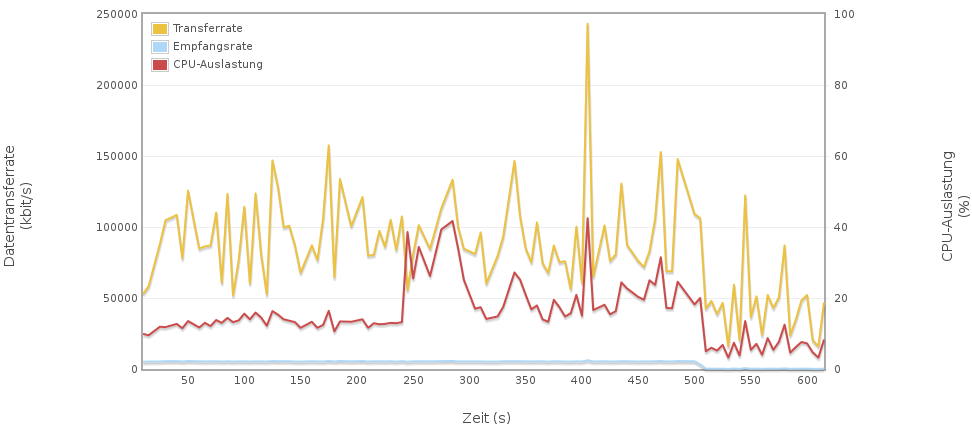
\includegraphics[width=\textwidth]{img/nack/nack_server2.png}
	\caption{\centering Gebündeltes Abweisen von Nachrichten - Verlauf der Transfer-, Empfangsrate und Verlauf der CPU-Last auf dem RabbitMQ-Server}
	\label{fig:nack-server2}
\end{figure}
\end{frame}

\begin{frame}{Angriff - Gebündeltes Abweisen von Nachrichten}	
\begin{figure}[!htb]
	\centering
	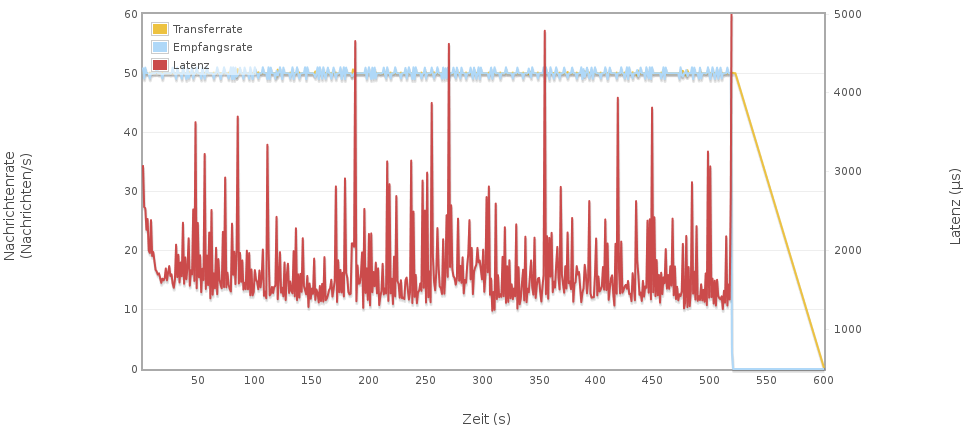
\includegraphics[width=\textwidth]{img/nack/nack_scenario.png}
	\caption{\centering Gebündeltes Abweisen von Nachrichten - Verlauf der Transfer-, Empfangsrate und Verlauf der Latenz im Anwendungsszenario}
	\label{fig:nack-scenario}
\end{figure}
\end{frame}

%-------------------------------------------------------%
% ---------------- Queue-Churning --------------------- %
%-------------------------------------------------------%
\begin{frame}[t]{Angriff - Queue-Churning}
\begin{description}
	\item[Aktion:]
		\begin{enumerate}
			\item Client erzeugt fortlaufend neue Queues bis zum Erreichen eines Schwellwertes
			\item \textbf{OPTIONAL} Client sendet Nachrichten an Queue 
			\item Client löscht schlagartig alle Queues
		\end{enumerate}  \smallskip
	\item[Ziel:] CPU, RAM \smallskip
	\item[Ansatz:] Server muss Überreste der Queue beseitigen, während bereits neue Queues erzeugt werden.
\end{description}
\end{frame}

\begin{frame}{Angriff - Queue-Churning}
\begin{figure}[!htb]
	\centering
	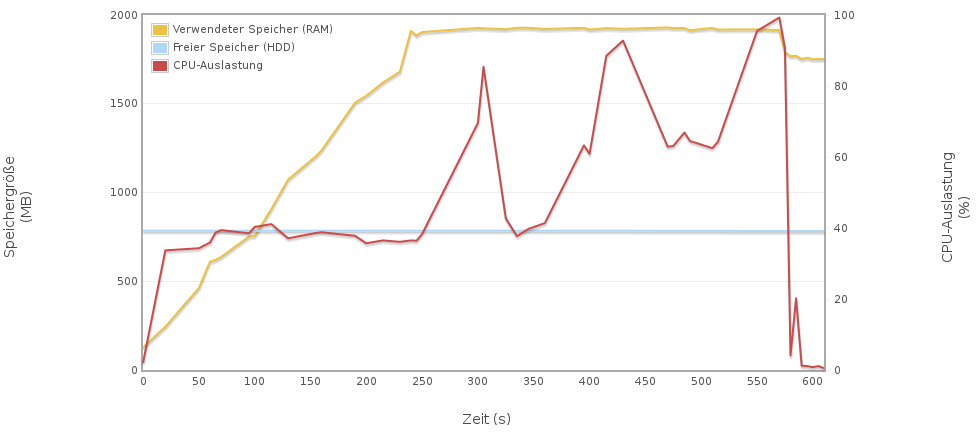
\includegraphics[width=\textwidth]{img/queue/queue_server1.png}
	\caption{\centering Queue-Churning - Verlauf des Speicherbedarfs für RAM/HDD und Verlauf der CPU-Last auf dem RabbitMQ-Server}
	\label{fig:queue-server1}
\end{figure}
\end{frame}
		
\begin{frame}{Angriff - Queue-Churning}
\begin{figure}[!htb]
	\centering
	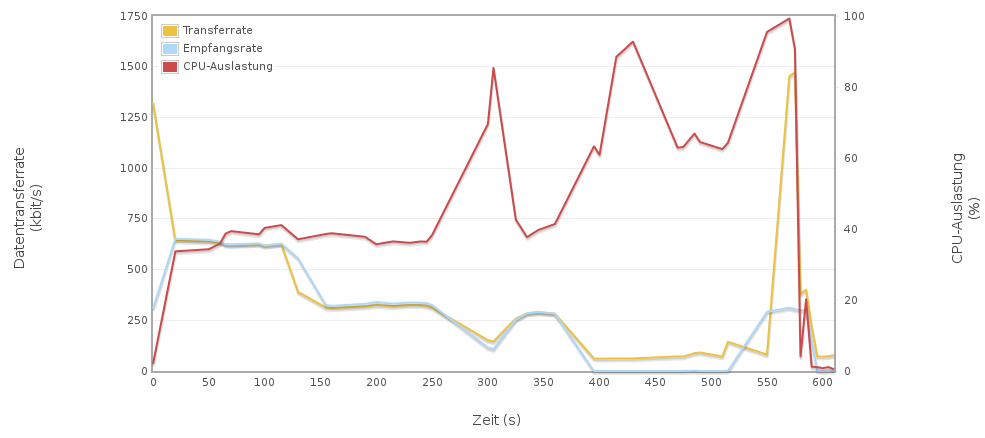
\includegraphics[width=\textwidth]{img/queue/queue_server2.png}
	\caption{\centering Queue-Churning - Verlauf der Transfer-, Empfangsrate und Verlauf der CPU-Last auf dem RabbitMQ-Server}
	\label{fig:queue-server2}
\end{figure}
\end{frame}
	
\begin{frame}{Angriff - Queue-Churning}	
\begin{figure}[!htb]
	\centering
	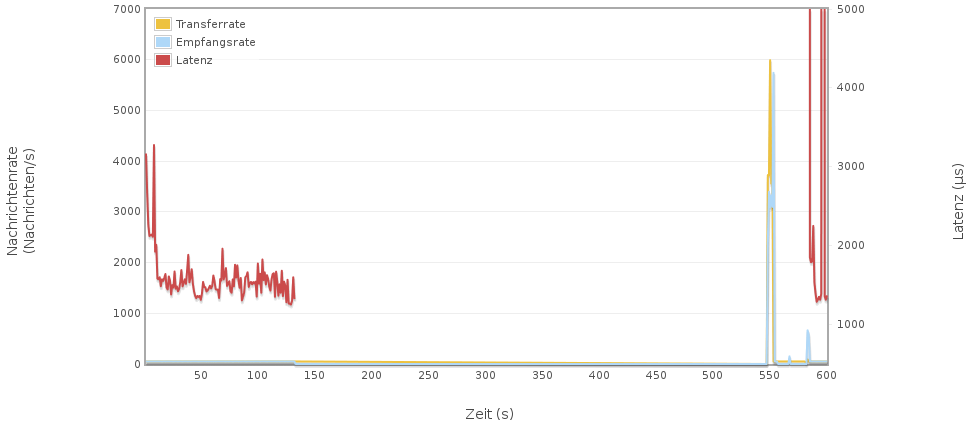
\includegraphics[width=\textwidth]{img/queue/queue_scenario.png}
	\caption{\centering Queue-Churning - Verlauf der Transfer-, Empfangsrate und Verlauf der Latenz im Anwendungsszenario}
	\label{fig:queue-scenario}
\end{figure}
\end{frame}




%-------------------------------------------------------%
% ------------------ Handshake-Trickle ---------------- %
%-------------------------------------------------------%
\begin{frame}[t]{Angriff - Handshake-Trickle}
\begin{description}
	\item[Aktion:]
		\begin{enumerate}
			\item Mehrere Clients starten einen Verbindungsaufbau zum Server
			\item Handshake wird in jeder Phase künstlich pausiert
			\item Clients schließen Verbindung
			\item Close-Handshake wird ebenfalls künstlich verlangsamt 
		\end{enumerate} \smallskip
	\item[Ziel:] Unerwartetes Verhalten seitens des Server  \smallskip
	\item[Ansatz:] Server muss für jeden begonnen Handshake Ressourcen zum Zustand des Verbindungsaufbaues bzw. Verbindungsabbaues allokieren.
\end{description}
\end{frame}

\begin{frame}{Angriff - Handshake-Trickle}
\begin{figure}[!htb]
	\centering
	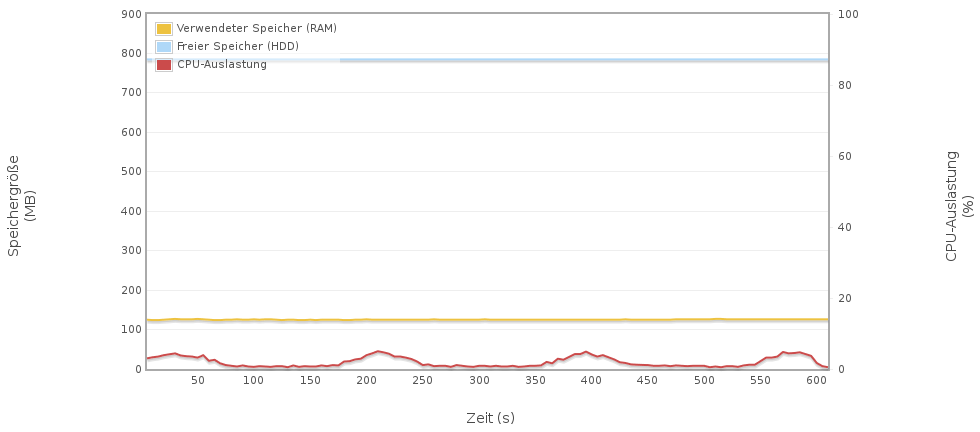
\includegraphics[width=\textwidth]{img/handshake/handshake_server1.png}
	\caption{\centering Handshake-Trickle - Verlauf des Speicherbedarfs für RAM/HDD und Verlauf der CPU-Last auf dem RabbitMQ-Server}
	\label{fig:handshake-server1}
\end{figure}
\end{frame}

\begin{frame}{Angriff - Handshake-Trickle}		
\begin{figure}[!htb]
	\centering
	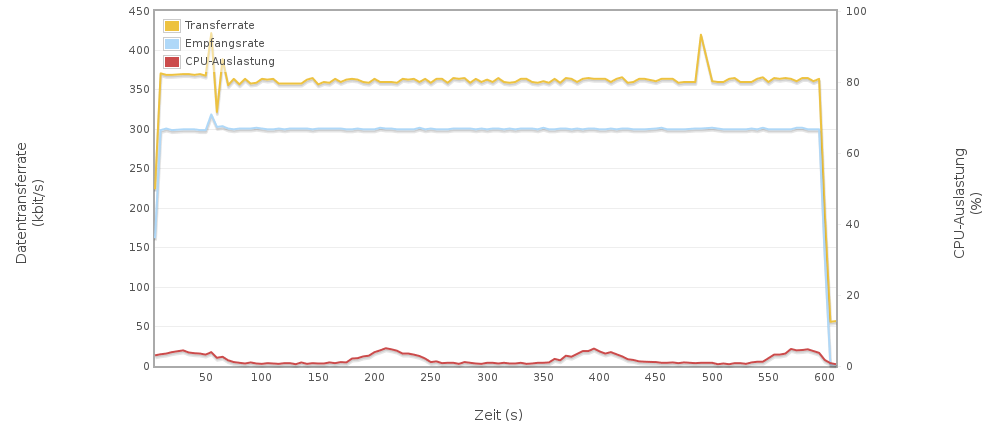
\includegraphics[width=\textwidth]{img/handshake/handshake_server2.png}
	\caption{\centering Handshake-Trickle - Verlauf der Transfer-, Empfangsrate und Verlauf der CPU-Last auf dem RabbitMQ-Server}
	\label{fig:handshake-server2}
\end{figure}
\end{frame}

\begin{frame}{Angriff - Handshake-Trickle}		
\begin{figure}[!htb]
	\centering
	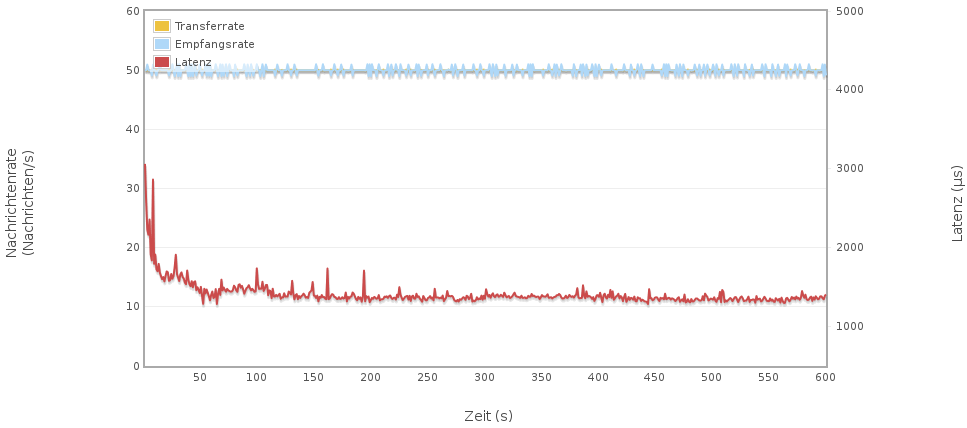
\includegraphics[width=\textwidth]{img/handshake/handshake_scenario.png}
	\caption{\centering Handshake-Trickle - Verlauf der Transfer-, Empfangsrate und Verlauf der Latenz im Anwendungsszenario}
	\label{fig:handshake-scenario}
\end{figure}
\end{frame}


%-------------------------------------------------------%
% ------------------ Heartbeat-Flooding --------------- %
%-------------------------------------------------------%
\begin{frame}[t]{Angriff - Heartbeat-Flooding}
\begin{description}
	\item[Aktion:]
		\begin{enumerate}
			\item Mehrere Clients öffnen Connections zum Server
			\item Clients stellen dabei Anfrage den Heartbeat herunterzusetzen
		\end{enumerate} \smallskip
	\item[Ziel:] CPU, Netzwerkbandbreite  \smallskip
	\item[Ansatz:] Server muss bei der Hälfte des angeforderten Timeouts einen Heartbeat an die Clients senden.
\end{description}
\end{frame}

\begin{frame}{Angriff - Heartbeat-Flooding}
\begin{figure}[!htb]
	\centering
	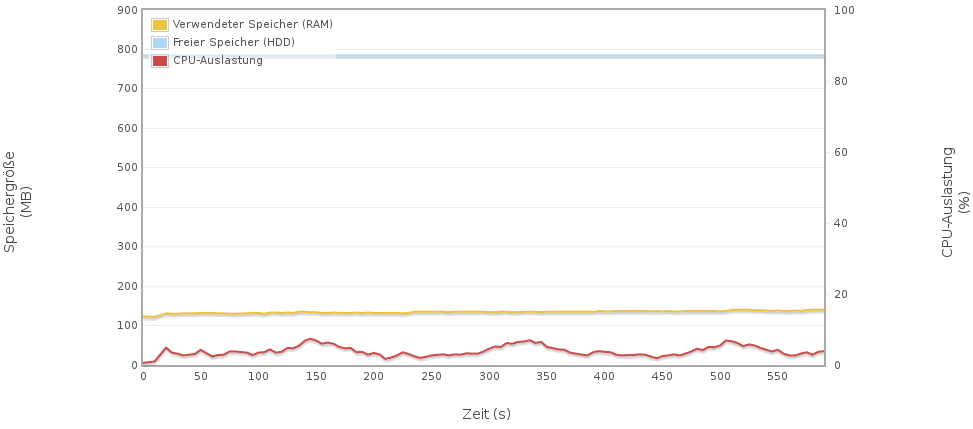
\includegraphics[width=\textwidth]{img/heartbeat/heartbeat_server1.png}
	\caption{\centering Heartbeat-Flooding - Verlauf des Speicherbedarfs für RAM/HDD und Verlauf der CPU-Last auf dem RabbitMQ-Server}
	\label{fig:heartbeat-server1}
\end{figure}
\end{frame}
	
\begin{frame}{Angriff - Heartbeat-Flooding}	
\begin{figure}[!htb]
	\centering
	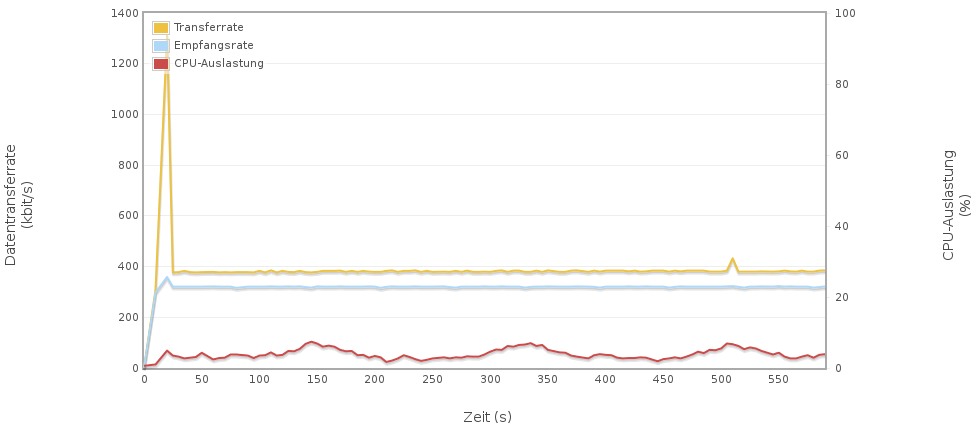
\includegraphics[width=\textwidth]{img/heartbeat/heartbeat_server2.png}
	\caption{\centering Heartbeat-Flooding - Verlauf der Transfer-, Empfangsrate und Verlauf der CPU-Last auf dem RabbitMQ-Server}
	\label{fig:heartbeat-server2}
\end{figure}
\end{frame}
	
\begin{frame}{Angriff - Heartbeat-Flooding}
\begin{figure}[!htb]
	\centering
	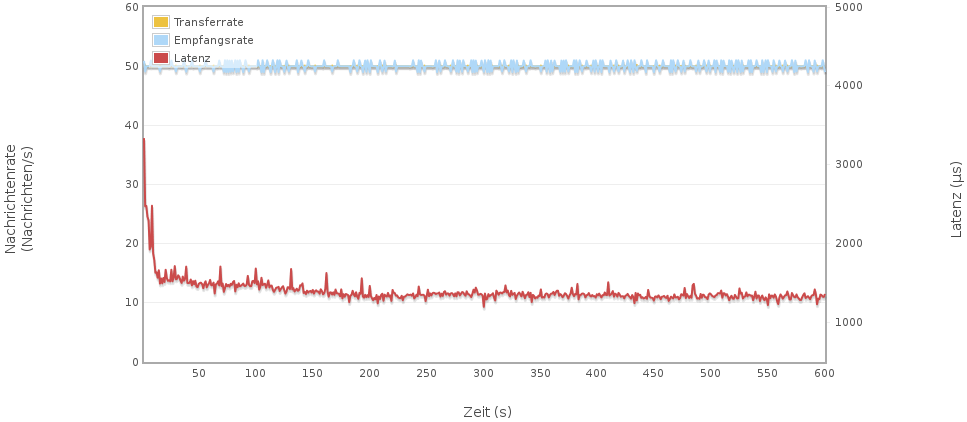
\includegraphics[width=\textwidth]{img/heartbeat/heartbeat_scenario.png}
	\caption{\centering Heartbeat-Flooding - Verlauf der Transfer-, Empfangsrate und Verlauf der Latenz im Anwendungsszenario}
	\label{fig:heartbeat-scenario}
\end{figure}
\end{frame}


%-------------------------------------------------------%
% ---------------- TCP-Connection-Droppin ------------- %
%-------------------------------------------------------%
\begin{frame}[t]{Angriff - TCP-Connection-Dropping}
\begin{description}
	\item[Aktion:]
		\begin{enumerate}
			\item Client öffnet Connection zum Server mit max. Heartbeat
			\item Extrahiert hierbei TCP-Socket
			\item Deaktiviert Keep-Alive, Aktiviert SO\_Linger
			\item Schließt TCP-Socket; Firewall blockiert RST-Paket
		\end{enumerate} \smallskip
	\item[Ziel:] RAM, Socketdeskriptoren \smallskip
	\item[Ansatz:] Server muss für jede \glqq offene\grqq\ Verbindung Ressourcen bereitstellen. Alle Mechanismen zur Erkennung der toten Verbindung werden verzögert oder deaktiviert.
\end{description}
\end{frame}

\begin{frame}{Angriff - TCP-Connection-Dropping}
\begin{figure}[!htb]
	\centering
	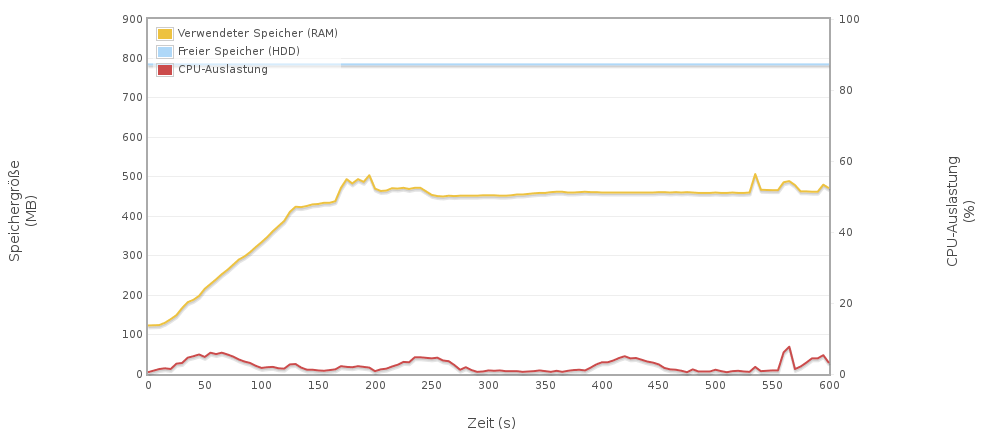
\includegraphics[width=\textwidth]{img/tcpdrop/tcpdrop_server1.png}
	\caption{\centering TCP-Connection-Dropping - Verlauf des Speicherbedarfs für RAM/HDD und Verlauf der CPU-Last auf dem RabbitMQ-Server}
	\label{fig:tcpdrop-server1}
\end{figure}
\end{frame}
	
\begin{frame}{Angriff - TCP-Connection-Dropping}
\begin{figure}[!htb]
	\centering
	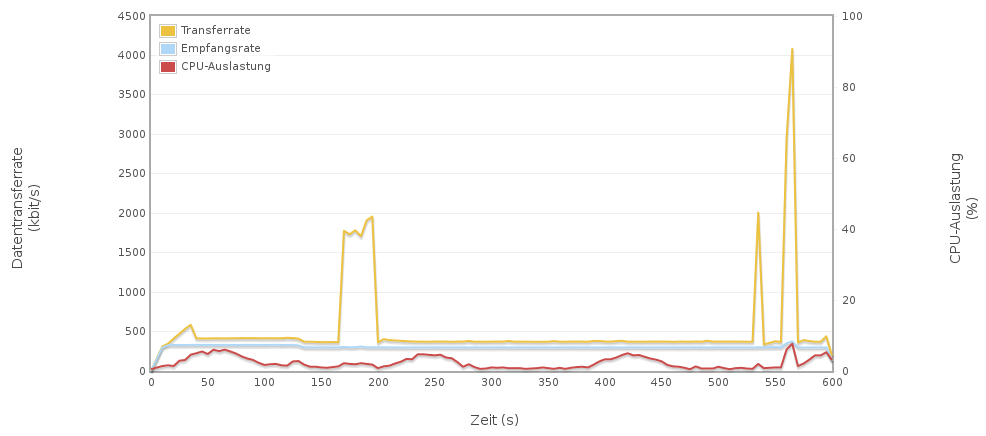
\includegraphics[width=\textwidth]{img/tcpdrop/tcpdrop_server2.png}
	\caption{\centering TCP-Connection-Dropping - Verlauf der Transfer-, Empfangsrate und Verlauf der CPU-Last auf dem RabbitMQ-Server}
	\label{fig:tcpdrop-server2}
\end{figure}
\end{frame}

\begin{frame}{Angriff - TCP-Connection-Dropping}
\begin{figure}[!htb]
	\centering
	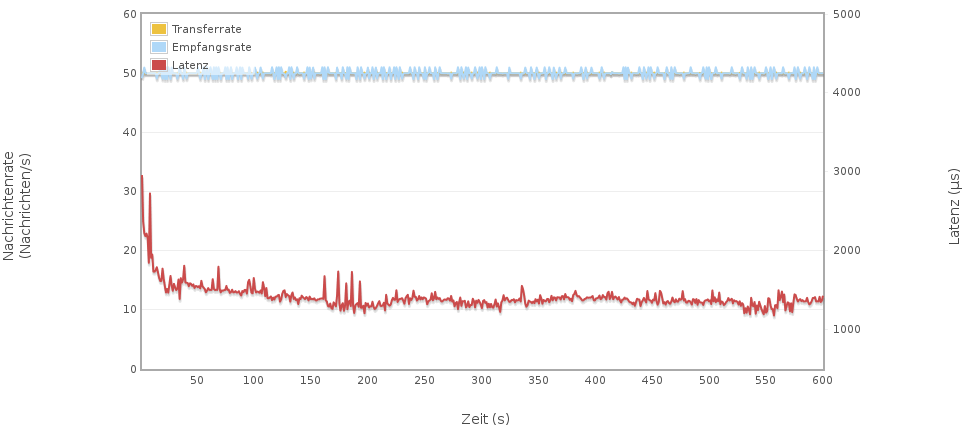
\includegraphics[width=\textwidth]{img/tcpdrop/tcpdrop_scenario.png}
	\caption{\centering TCP-Connection-Dropping - Verlauf der Transfer-, Empfangsrate und Verlauf der Latenz im Anwendungsszenario}
	\label{fig:tcpdrop-scenario}
\end{figure}
\end{frame}


%################################################################%
% ####################### Abschluss ############################ %
%################################################################%
\section{Abschluss}

\begin{frame}[t]{Umsetzung - Mögliche Angriffsvektoren}
	\begin{itemize}
		\item Viele Verbindungen \uncover<2->{\textcolor{green}{+ Viele Channel} \ok}
		\item Bruteforce-Attacke auf Benutzercredentials \uncover<2->{\nok}
		\item Hohe Datenrate (viele kleine, wenig große Nachrichten) \uncover<2->{\ok}
		\item Große Header, kleiner Payload \uncover<2->{\ok}
		\item Langsamer Verbindungsaufbau  \uncover<2->{\textcolor{green}{+ Verbindungsabbau} \ok}
		\item Unvollständiger Verbindungsaufbau \uncover<2->{\textcolor{blue}{\Large\textasciitilde}}
		\item Pause im Protokollablauf \uncover<2->{\textcolor{blue}{\Large\textasciitilde}}
		\item<2-> \textcolor{green}{Queue-Churning}
		\item<2-> \textcolor{green}{Heartbeat-Flooding}
		\item<2-> \textcolor{green}{Transaktionen}
		\item<2-> \textcolor{green}{Ausnutzen Message-Response}
	\end{itemize}	
\end{frame}
  
\begin{frame}[t]{Zusammenfassung}
	\begin{itemize}
		\item Umfangreiche Angriffsszenarien realisiert\\
			\ding{229} Genügend Potenzial für weitere Angriffsszenarien
		\item Angefragte Konfiguration durch Client oft ausschlaggebend \\
			\ding{229} Prefetching, Framegröße, Heartbeat, ...
		\item Konfigurierte Ressourcen-Limits werden teilweise ignoriert \\
			\ding{229} RAM bei Queues, Transaktionen\medskip
	\end{itemize}	
\end{frame}

\begin{frame}[t]{Fazit \& Empfehlung}
	\begin{itemize}
		\item Konfigurierte Ressourcen-Limits sollten verbindlich sein
		\item Konfigurationsspielraum für Clients sollte auf Einsatzgebiet eingeschränkt werden\\
		\ding{229} Anzahl Queues, Channel, Prefetching, Framegröße, Headergröße, Heartbeat, Transaktionsgröße
	\end{itemize}
	\uncover<2->{
	\begin{center}
		\large 
		RabbitMQ ist stabiler Messagebroker, der in Standardkonfiguration jedoch nicht gefahrlos verwendet werden kann.
	\end{center}}
\end{frame}

\begin{frame}{Kontakt}
	\Large
	\Letter\, \textsl{\href{mailto:marcel.mielke@stud.htwk-leipzig.de}{marcel.mielke@stud.htwk-leipzig.de}}\bigskip\\
	\Letter\, \textsl{\href{mailto:philipp.sieder@stud.htwk-leipzig.de}{philipp.sieder@stud.htwk-leipzig.de}}
	
\end{frame}

%################################################################

\plain{Fragen?}

\end{document}
